\chapter{Platform}

\begin{figure}[H]
	\centering
	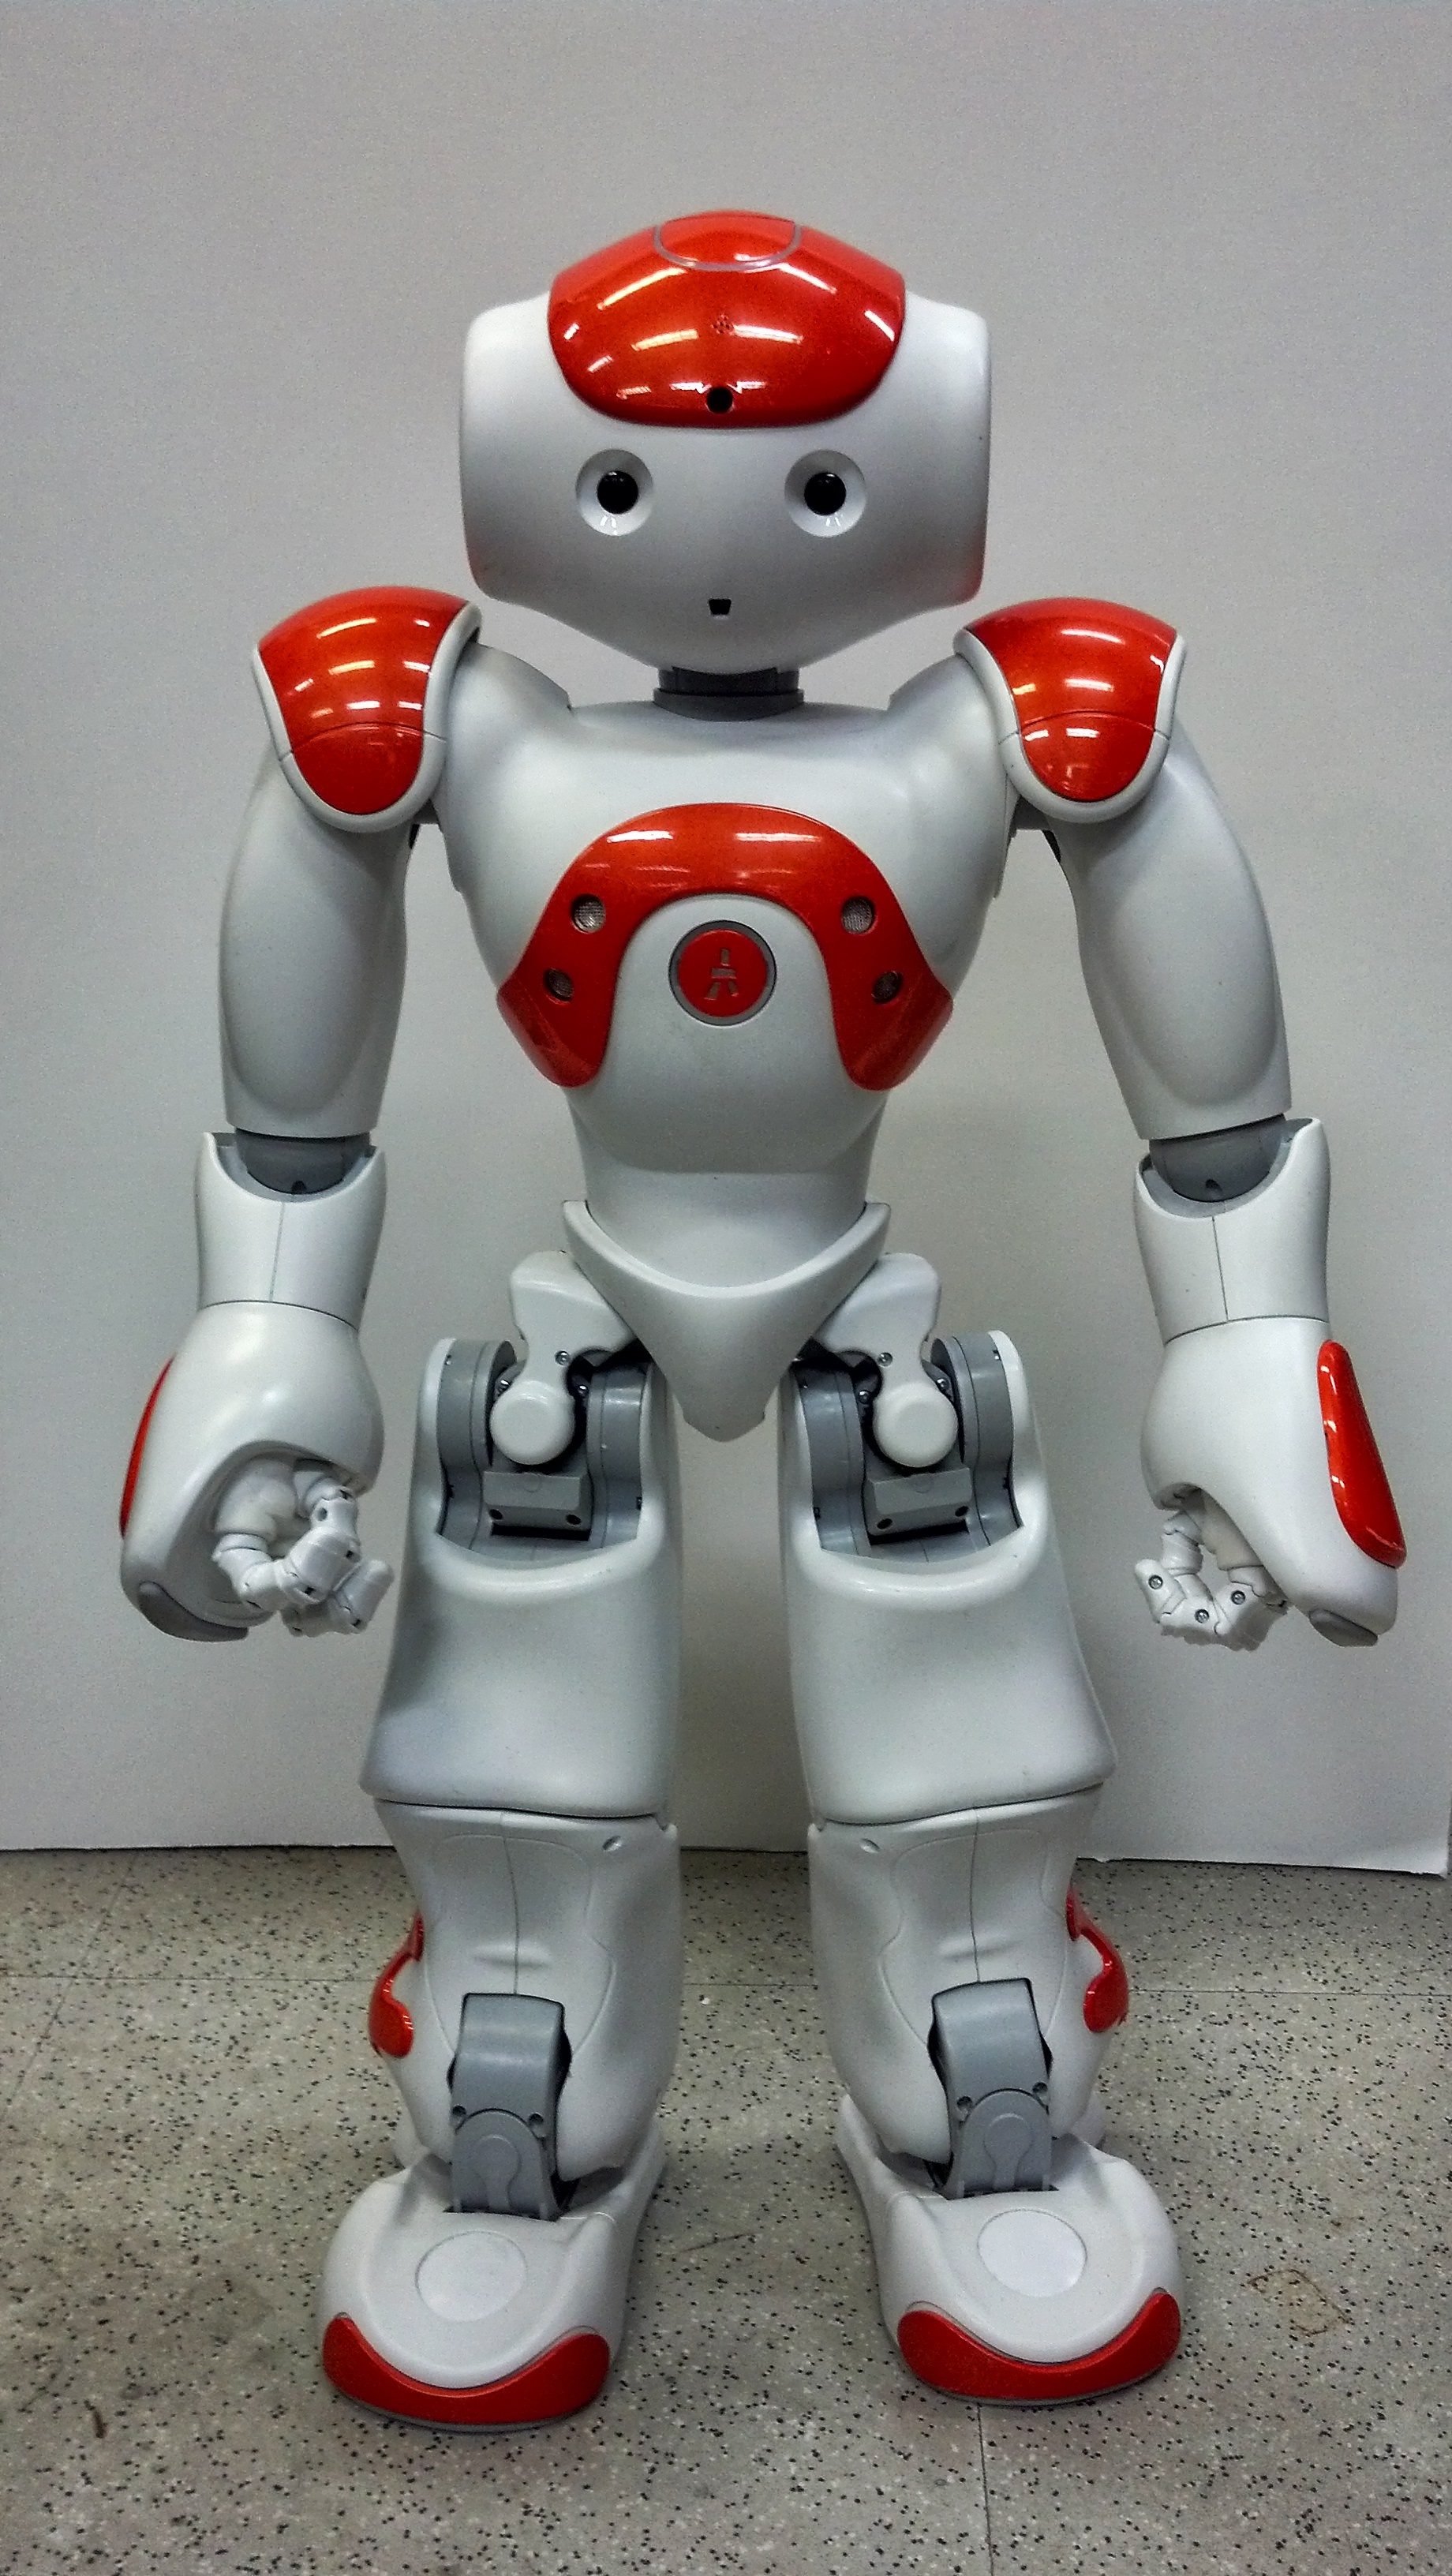
\includegraphics[width=0.35\textwidth]{nao1.jpg}
	\caption
	{Nao robot at Control/Robotics Research Lab}
	\label{fig:nao1}
\end{figure}

The platform utilized on this project was the Nao humanoid experimental robotic platform by Aldebaran Robotics. It is a 25 degree-of-freedom humanoid mobile manipulator with two HD cameras, two ultrasonic distance sensors, four microphones, one three-axis accelerometer, two one-axis gyroscopes, and four force sensors in each foot. The platform is programmed using a framework called NAOqi allowing development using various languages including C++ and Python. 

Two ultrasonic sensors in the chest allowed for distance measurements to occlusions. The transmitters are mounted at an angle of 20 degrees from the forward direction of the Nao and the receivers are mounted at 25 degrees. They have a 60 degree viewing angle with a detection range between 0.25 and 2.55 meters with a 1 cm resolution.

\begin{figure}[h]
	\centering
	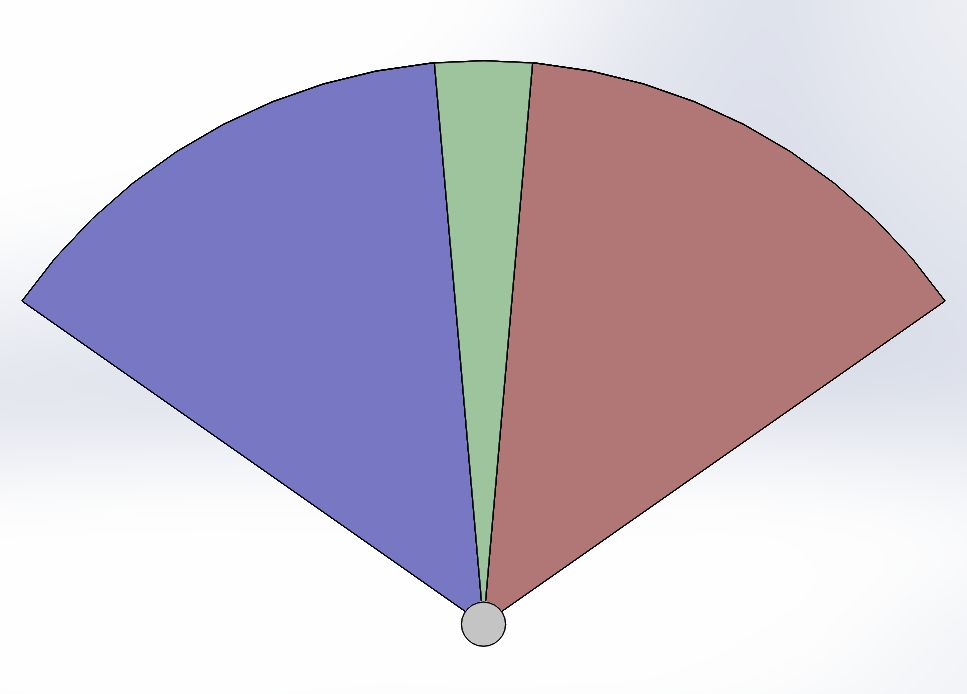
\includegraphics[width=0.35\textwidth]{sonar1.jpg}
	\caption
	[Nao sonar cones.]
	{Nao sonar cones. The left cone is shown in blue and the right cone is shown in red. The green cone shows the overlap between the two.}
	\label{fig:sonar1}
\end{figure}

As shown in Figure \ref{fig:sonar1} the regions covered by the two ultrasonic sensors overlap. As the sensors do not report the angular position of the occlusion within the cone, uncertainty about the location of detected objects is high as they could be anywhere within the sonar cone.

The motion API for the Nao takes three different velocity commands, forward, lateral, and angular, in terms of fraction of maximum step length and step frequency. The maximum step length is 8 cm forward, 16 cm laterally, and 0.523 radians angularly. The maximum step frequency is 2.381 Hz. Due to a stability controller in the built-in gaiting algorithm for the Nao, it takes 0.8 seconds for the robot to react to new commands. At maximum step frequency, this equates to about 2 steps. \cite{naodoc_motion1}

Talk about built in red ball tracking for head that returns range and bearing estimates of a red ball 6 cm in diameter.

